%------------------------------------------------------------------------------
% Template file for the submission of papers to IUCr journals in LaTeX2e
% using the iucr document class
% Copyright 1999-2013 International Union of Crystallography
% Version 1.6 (28 March 2013)
%------------------------------------------------------------------------------

\documentclass{iucr}
% \documentclass[preprint]{iucr}              % DO NOT DELETE THIS LINE
\usepackage{bm}
% \usepackage{graphicx}
% \usepackage{tabularx}
% \usepackage{subfigure}
% \usepackage{afterpage}
% \usepackage{sansmath}
\usepackage{mathtools}
% \usepackage{parskip}
% \usepackage{tikz}
% \usepackage{tikzorbital}
% \usepackage{setspace}
% \usepackage{xcolor}
\usepackage{amssymb}
% \usepackage{bm}
\usepackage{amsmath}
% \usepackage{fancyhdr}
% \usepackage{rotating}
\usepackage{siunitx}
\usepackage[hyphens,spaces,obeyspaces]{url}
\usepackage{color}
\usepackage{siunitx}
\usepackage[hyphens,spaces,obeyspaces]{url}
\usepackage{color}
%\usepackage{cprotect}
\usepackage{textgreek}
\usepackage[normalem]{ulem}
\usepackage{makecell}
\usepackage{cancel}
\usepackage{empheq}
\usepackage[usenames,dvipsnames]{xcolor}

\definecolor{darkblue}{rgb}{0.0, 0.0, 0.55}
\definecolor{cyan(process)}{rgb}{0.0, 0.72, 0.92}

\newcommand{\todo}[1]{{\color{red}[TODO: "#1'']}}
\newcommand{\inblue}[1]{{\color{blue}#1}}
\newcommand{\cyan}[1]{{\color{cyan(process)}#1}}
\newcommand{\inred}[1]{{\color{red}#1}}
\newcommand{\ingreen}[1]{{\color{green}#1}}

\makeatletter
\@ifclasswith{iucr}{preprint}{
\newcommand{\whencolumns}[2]{#1}
}{
\newcommand{\whencolumns}[2]{#2}
}
\makeatother

     %-------------------------------------------------------------------------
     % Infobrmation about journal to which submitted
     %-------------------------------------------------------------------------
     \journalcode{X}              % Indicate the journal to which submitted
                                  %   A - Acta Crystallographica Section A
                                  %   B - Acta Crystallographica Section B
                                  %   C - Acta Crystallographica Section C
                                  %   D - Acta Crystallographica Section D
                                  %   E - Acta Crystallographica Section E
                                  %   F - Acta Crystallographica Section F
                                  %   J - Journal of Applied Crystallography
                                  %   M - IUCrJ
                                  %   S - Journal of Synchrotron Radiation

\begin{document}                  % DO NOT DELETE THIS LINE

     %-------------------------------------------------------------------------
     % The introductory (header) part of the paper
     %-------------------------------------------------------------------------

     % The title of the paper. Use \shorttitle to indicate an abbreviated title
     % for use in running heads (you will need to uncomment it).

\title{\cyan{Diffracted amplitudes} for perfect crystals derived from solutions of Takagi-Taupin equations \cyan{and numerical implementation in the \texttt{crystalpy} library.}}
% * <msanchezdelrio@gmail.com> 2018-09-25T09:38:50.716Z:
%
% ^.
%\shorttitle{Short Title}

     % Authors' names and addresses. Use \cauthor for the main (contact) author.
     % Use \author for all other authors. Use \aff for authors' affiliations.
     % Use lower-case letters in square brackets to link authors to their
     % affiliations; if there is only one affiliation address, remove the [a].

\cauthor[a]{Jean-Pierre}{Guigay}{guigay@esrf.eu}{address if different from \aff}
\author[a]{Manuel}{Sanchez del Rio}


\aff[a]{European Synchrotron Radiation Facility, 71 Avenue des Martyrs F-38000 Grenoble \country{France}}


     % Use \shortauthor to indicate an abbreviated author list for use in
     % running heads (you will need to uncomment it).

%\shortauthor{Soape, Author and Doe}

     % Use \vita if required to give biographical details (for authors of
     % invited review papers only). Uncomment it.

%\vita{Author's biography}

     % Keywords (required for Journal of Synchrotron Radiation only)
     % Use the \keyword macro for each word or phrase, e.g. 
     % \keyword{X-ray diffraction}\keyword{muscle}

%\keyword{keyword}

     % PDB and NDB reference codes for structures referenced in the article and
     % deposited with the Protein Data Bank and Nucleic Acids Database (Acta
     % Crystallographica Section D). Repeat for each separate structure e.g
     % \PDBref[dethiobiotin synthetase]{1byi} \NDBref[d(G$_4$CGC$_4$)]{ad0002}

%\PDBref[optional name]{refcode}
%\NDBref[optional name]{refcode}

\maketitle                        % DO NOT DELETE THIS LINE

\begin{synopsis}
The Takagi-Taupin equations are solved in its simpler form (zero deformation) and equations of the diffracted and transmitted amplitudes are obtained. Then, the case of a multilayered crystal is discussed using a matrix model. 
\end{synopsis}

% \today

\begin{abstract}

The Takagi-Taupin equations are solved in its simpler form (zero deformation) and equations of the diffracted and transmitted amplitudes are obtained. \cyan{The case of multilayered crystals is discussed using a matrix model. The equations are implemented in a python library \texttt{cryslalpy} adapted for numeric applications like reflectivity calculations and ray-tracing.} 

\end{abstract}


     %-------------------------------------------------------------------------
     % The main body of the paper
     %-------------------------------------------------------------------------
     % Now enter the text of the document in multiple \section's, \subsection's
     % and \subsubsection's as required.

\section{Introduction}
\label{sec:Intro}

\cyan{
Almost every synchrotron radiation beamline operating at hard X-rays makes use of perfect crystals.  
Most beamlines use crystal monochromators, typically in the DCM (double crystal monochromator) mode, but polychromators or single crystal Laue monochromators can be also found. In addition, crystal analyzers are used in most spectroscopy beamlines. 
Beamline simulation tools used for the design, optimization and commissioning of synchrotron instrumentation implement in software the equations to calculate reflectivities of perfect crystals. The theory of diffraction (see \cite{authierbook} for a complete reference) puts the bases of all numeric implementations. 

There are lots of simulation tools implementing the equations of the dynamical theory in different forms. This variate scenario is even more complex if we consider that the calculation of the crystal structure factor, which is an essential ingredient to calculate diffracted amplitudes and intensities, is obtained from tabulated scattering functions of multiple origin. The wide menu of available methods and tools can be found even in the single suite OASYS \cite{codeOASYS}, that provides multiple solutions for calculating diffraction profiles of crystals (e.g. INPRO\footnote{\texttt{https://github.com/oasys-kit/xoppy\_externa\_codes/tree/master/src/INPRO}}, CRYTSTAL\cite{codeCRYSTAL}, X-RAY Server \cite{codeXRAYserver}), as well as beamline simulation tools (based on the ray tracing code SHADOW\cite{codeSHADOW}) and physical wave-optics simulations (with SRW\cite{codeSRW, codeSRWcrystals}). This scenario has heritaged decades of developments and have witnessed several synchrotron radiation generations. The work presented here looks into the future to improve this situation. We have two objectives: derive the equations of the crystal reflectivities from first principles and implementing them in a software library.

In section~\ref{sec:TT} we derive the Takagi-Taupin (TT) equations \cite{Takagi1962, Taupin, Taupin1967} equations. In section~\ref{sec:TTsolutions} we solve the TT equations for a plane undeformed-crystal, giving four fundamental results: the diffracted and forward-diffracted (or transmitted) amplitudes for a crystal set in Bragg (reflection) and Laue (transmission) geometries. The diffracted amplitudes constitute the elements of the transfer matrices (section~\ref{sec:matrices}), useful to calculate systems of layered crystals and multilayers. Section~\ref{sec:crystalpy} is dedicated to the software implementation (library \texttt{crystalpy}, discussing some details and applications.
 }
 
 
%%%%%%%%%%%%%%%%%%%%%%%%%%%%%%%%%%%%%%%%%%%%%%%%%%%%
%
%%%%%%%%%%%%%%%%%%%%%%%%%%%%%%%%%%%%%%%%%%%%%%%%%%%%
\section{The Takagi-Taupin equations for a plane incident wave}
\label{sec:TT}

Let us start with the Helmholtz equation in a crystal

\begin{equation}
\label{eq:helmholz}
    \Delta \Psi + k^2 (1+\chi) \Psi = 0,
\end{equation}
with $\chi$ the electric susceptibility (refraction index $n=(1+\chi)^{1/2}$) and $\Psi$ the time-independent electric field inside the crystal. In a crystal, the electric susceptibility can be expanded in Fourier series,
\begin{equation}
\label{eq:chi}
    \chi = \sum_{\textbf{h}} \chi_h \exp(i \textbf{h} . \textbf{r}),
\end{equation}
where $\bf{h}$ is the reciprocal lattice vector (with modulus $|\textbf{h}|=2\pi/d_\text{hkl}$, being $d_\text{hkl}$ the d-spacing of the hkl reflection), and the sum goes over all reciprocal vectors $|\textbf{h}|$ with possible hkl Miller indices. If a single reflection $\bf{h}$ is considered, only the terms $\bf{0}$, $\bf{h}$ and $\bf{-h}$ are non-zero, 
\begin{equation}
\label{eq:chisimple}
    \chi = \chi_0 + \chi_{h} \exp(i \textbf{h} . \textbf{r}) + \chi_{-h} \exp(-i \textbf{h} . \textbf{r}).
\end{equation}

The x-ray wavefield inside the crystal is expressed as the sum of two modulated plane waves
\begin{equation}
\label{eq:wavefield}
    \Psi(\textbf r) = D_0(\textbf r) e^{i \textbf k_0 . \textbf r} + D_h(\textbf r) e^{i \textbf k_h . \textbf r},
\end{equation}
with amplitudes\footnote{
\cyan{
Note that equation~(\ref{eq:wavefield}) expresses the field inside the crystal along incident and diffracted directions. However,the exact choice of  these directions may vary: we opted for a vector $\textbf{k}_0$ along the direction of the incident wave, and $\textbf{k}_h$ defined later. We could use incident and diffracted vectors defined in other ways, in such a way that the ``differences" are absorbed in the amplitudes $D_{0,h}$. In appendix~\ref{appendix:rotating}, we explore another alternative}
} $D_{0,h}(\textbf r)$.
The vector $\textbf{k}_h$ can be defined, without lost of generality, as $\textbf k_h=\textbf k_0 + \textbf h$. 
The wavevector modulus is $k \equiv |\textbf{k}_0|=2\pi/\lambda$, where $\lambda$ is x-ray wavelength in vacuum. Note that, in general, $ |\textbf{k}_h| \ne k$. Only for a direction along the geometrical Bragg position ($\textbf{k}_0=\textbf{k}_0^B$), the Laue equations ($\textbf{k}_h^B=\textbf{k}_0^B+\textbf{h}$) holds, and $|\textbf{k}_0^B|=|\textbf{k}_h^B|$. This definition implies that, in general, the outgoing Bragg wave outside the crystal} is not \cyan{ along the direction of $\textbf{k}_h$.}


% The Takagi-Taupin equations are obtained 
To obtain the Takagi-Taupin equations (TT) we insert the equations~(\ref{eq:chisimple}) and (\ref{eq:wavefield}) in (\ref{eq:helmholz}) and consider two approximations. One supposes $D_{0,h}$ to be slowly varying amplitudes, thus neglecting the 2$^{\text{nd}}$ order derivatives of $D_{0,h}$,  so that
\begin{subequations}
\label{eq:approxslowlyvarying}
\begin{align}
&(\Delta + k^2)[D_{0,h}(\textbf{r}) \exp(i\textbf{k}_{0,h} . \textbf{r})] \approx \nonumber  \\
&\exp(i\textbf{k}_{0,h} . \textbf{r}) [2 i \textbf{k}_{0,h} . \nabla D_{0,h} + (k^2 - k^2_{0,h}) D_{0,h}].
\end{align}
\end{subequations}
The second approximation neglects two
\footnote{\cyan{
in such a way that the two-waves approximation is maintained. In appendix~\ref{appendix:rotating} an alternative choice of the incident and diffracted directions is made, and in this case these two terms are zero.
}}
of the six terms in $\chi \Psi$
\begin{subequations}
\label{eq:approxchiPsi}
\begin{align}
\chi\Psi =&
\chi_0 D_0 \exp(i \textbf{k}_0 . \textbf{r}) +
\chi_0 D_h \exp(i \textbf{k}_h . \textbf{r}) +\\
&\chi_h D_0 \exp(i \textbf{k}_h . \textbf{r}) +
\cancelto{\approx 0}{\chi_h D_h \exp(i (\textbf{k}_0+2\textbf{h}) . \textbf{r})} +\\
&\cancelto{\approx 0}{\chi_{-h} D_0 \exp(i (\textbf{k}_0 - 2 \textbf{h}) .\textbf{r})} +
\chi_{-h} D_h \exp(i \textbf{k}_0 . \textbf{r}) .
\end{align}
\end{subequations}
We obtain in this way the TT equations 
\begin{subequations}
\label{eq:TTvector}
\begin{align}
2 i \textbf{k}_0 . \nabla D_0 + \chi_0 k^2 D_0 + \chi_{-h} k^2 D_h =& 0; \\
2 i \textbf{k}_h . \nabla D_h + (k^2 - k_h^2 + \chi_0 k^2) D_h + \chi_{h} k^2 D_0 =& 0.
\end{align}
\end{subequations}

We define a parameter $\alpha$ that measures the deviation\footnote{
\cyan{Note that the $\alpha$ defined in \cite{ZachariasenBook} (equation [3.114b]) is the same as here but with opposite sign.  }
}
of the incident angle from the geometrical Bragg position as
\begin{equation}
\label{eq:alpha}
\alpha = \frac{k^2-k_h^2}{k^2} = \frac{k^2-(\textbf k_0 + \textbf h)^2}{k^2} = - \frac{\textbf h^2 + 2 \textbf k_0 . \textbf h}{k^2}.
% = 4 \sin \theta_B (\sin \theta - \sin \theta_B) \approx 2 (\theta-\theta_B) \sin 2\theta_B),
\end{equation}

In the ``rotating crystal mode" $\alpha=4 \sin \theta_B (\sin \theta - \sin \theta_B) \approx 2 (\theta-\theta_B) \sin (2\theta_B)$, with $\theta$ the glancing angle on the reflective planes, and $\theta_B$ the Bragg angle ($h=2 k \sin\theta_B$, $\textbf k_0 . \textbf h = -2 k \sin\theta$). Note that the last approximation fails far from the Bragg position or if $\cos\theta_B \rightarrow 0$ (normal incidence)\cyan{, therefore the equation~\ref{eq:alpha} is used in the software}.
The TT equation become
\begin{subequations}
\label{eq:TTvectorAlpha}
\begin{align}
2 i \textbf{k}_0 . \nabla D_0 + \chi_0 k^2 D_0 + \chi_{-h} k^2 D_h =& 0; \\
2 i \textbf{k}_h . \nabla D_h + (\alpha + \chi_0) k^2 D_h + \chi_{h} k^2 D_0 =& 0.
\end{align}
\end{subequations}

A point in the diffraction plane (the plane containing $\textbf{k}_0$ and $\textbf{h}$) 
can be expressed with two oblique coordinates $(s_0,s_h)$ along the directions of the $\textbf k_0$ and $\textbf k_h$ (unit vectors $\hat{ \textbf{s}}_{0}$ and $\hat{ \textbf{s}}_{h}$, respectively). A generic spatial spatial position will also include a third \cyan{transverse} coordinate $\textbf{s}_t$ along an axis $\hat{\textbf{s}}_t=\hat{\textbf{s}}_0 \times \hat{\textbf{s}}_h$, therefore $\textbf r=(s_0,s_h,s_t)$. The director cosines are $\gamma_{0,h,t}=\cos(\textbf{n} , \hat{\textbf{s}}_{0,h,t}) \equiv \cos(\theta_{0,h,t})$. The equation of the crystal surface is $\gamma_0 s_0 + \gamma_h s_h + \gamma_t s_t=0$. For any point $\textbf r=(s_0,s_h,s_t)$ inside the crystal we introduce the path length $s$ \inred{of the incident ray going in this point}: this ray meets the crystal surface in the point of coordinates $(s'_0,s_h,s_t)$ such that $\gamma_0 s'_0+\gamma_h s_h + \gamma_t s_t=0$, so that 
\begin{equation}
\label{eq:s}
s = s_0 - s'_0 = s_0 + s_h \frac{\gamma_h}{\gamma_0} + s_t \frac{\gamma_t}{\gamma_0}.
\end{equation}

The simple relation $d s_0 = \nabla s_0 . [ d s_0 . \hat{\textbf{s}}_0 + d s_h \hat{\textbf{s}}_h + d s_t \hat{\textbf{s}}_t ]$ implies $\nabla s_0 . \hat{\textbf{s}}_0=1$ and $\nabla s_0 . \hat{\textbf{s}}_{h,t}=0$. Similarly, $\nabla s_h . \hat{\textbf{s}}_h=1$ and $\nabla s_h . \hat{\textbf{s}}_{0,t}=0$. Therefore, 
\begin{subequations}
\label{eq:equalities}
\begin{align}
\hat s_0 . \nabla D=
\hat s_0 . \left[ 
\frac{\partial D}{\partial s_0} \nabla s_0 + 
\frac{\partial D}{\partial s_h} \nabla s_h +
\frac{\partial D}{\partial s_t} \nabla s_t
\right] 
=& \frac{\partial D}{\partial s_0}
; \\
\hat s_h \nabla D =& 
\frac{\partial D}{\partial s_h}.
\end{align}
\end{subequations}

Using the approximation \todo{physical meaning, justify?}
\begin{equation}
\label{eq:approxKH}
\textbf k_h . \nabla D_h = |\textbf k_h| \frac{\partial D_h}{\partial s_h} \approx k \frac{\partial D_h}{ \partial s_h},
\end{equation}
we obtain from equations~(\ref{eq:TTvector})
\begin{subequations}
\label{eq:TT}
% \begin{align}
\begin{empheq}[box=\fbox]{align}
\frac{\partial D_0}{\partial s_0} =& \frac{ik}{2} \left[ \chi_0 D_0(s_0,s_h,s_t)+ \chi_{-h} D_h(s_0,s_h) \right]; \\
\frac{\partial D_h}{\partial s_h} =& \frac{ik}{2} \left[ (\chi_0 + \alpha) D_h(s_0,s_h,s_t)+ \chi_{h} D_0(s_0,s_h,s_t) \right],
% \end{align}
\end{empheq}
\end{subequations}
or in a more compact form
\begin{subequations}
\label{eq:TTcompact}
\begin{align}
\frac{\partial D_0}{\partial s_0} =& i u_0 D_0(s_0,s_h,s_t) + i u_{-h} D_h(s_0,s_h,s_t); \\
\frac{\partial D_h}{\partial s_h} =& i (u_0 + \alpha') D_h(s_0,s_h,s_t) + i u_{h} D_0(s_0,s_h,s_t),
\end{align}
\end{subequations}
where it has been used the notation $u_{0,h,-h}=(\pi/\lambda) \chi_{0,h,-h}$ and $\alpha' = (\pi/\lambda) \alpha$.



%%%%%%%%%%%%%%%%%%%%%%%%%%%%%%%%%%%%%%%%%%%%%%%%%%%%
%
%%%%%%%%%%%%%%%%%%%%%%%%%%%%%%%%%%%%%%%%%%%%%%%%%%%%
\section{Solutions of TT equations... \inred{as a function of $s$??}}
\label{sec:TTsolutions}

%%%%%%%%%%%%%%%%%%%%%%%%%%%%%%%%%%%%%%%%%%%%%%%%%%%%
%
%%%%%%%%%%%%%%%%%%%%%%%%%%%%%%%%%%%%%%%%%%%%%%%%%%%%

It is interesting to consider first the effects of refraction and absorption without Bragg diffraction. 
According to equation~(\ref{eq:TTcompact}a), the differential equation for the refracted wave is
\begin{equation}
\frac{\partial D_0^{\text{ref}}}{\partial s_0} = i u_0 D_0^{\text{ref}};
\end{equation}
its solutions are of the form $D_0^{\text{ref}}=f(s_h,s_t) \exp(i u_0 s_0)$, and the boundary condition is $D_0^{\text{ref}}=1$ for  $\gamma_0 s_0 + \gamma_h s_h + \gamma_t s_t=0$, from which $f(s_h,s_t)=\exp(i u_0 (s_h \gamma_h + s_t \gamma_t)/\gamma_0)$; therefore $D_0^{\text{ref}}= \exp(i u_0 s_0 + i u_0(s_h \gamma_h + s_t \gamma_t)/\gamma_0) \equiv \exp(i u_0 s)$, with $s=s_0+(s_h \gamma_h+s_t \gamma_t)/\gamma_0$.

We will now obtain the solutions of the TT equations depending on the single variable $s$, which means 
$\partial D_{0} / \partial  s_{0}=D'_{0}(s)$ and $\partial D_{h} / \partial s_{h}=D'_{h}(s)\gamma_h/\gamma_0$.
Defining $b=\gamma_0/\gamma_h$, the equations~(\ref{eq:TTcompact}) become
\begin{subequations}
\label{eq:TTlaue}
\begin{align}
D'_0(s) =& i u_0 D_0(s) + i u_{-h} D_h(s); \\
D'_h(s) =& i b (u_0 + \alpha') D_h(s) + i b u_{h} D_0(s).
\end{align}
\end{subequations}

It is convenient to introduce the functions $B_{0,h}(s)$ by setting
\begin{equation}
\label{eq:Bdefinition}
D_{0,h} = \exp \left( i s \frac{u_0 + b (u_0+\alpha')}{2} \right) B_{0,h} = \exp(i s (u_0+\omega)) B_{0,h},  
\end{equation}
with $\boxed{\omega=(b(u_0+\alpha')-u_0)/2}$. They are solutions of 
\begin{subequations}
\label{eq:TTinB}
\begin{align}
B'_0(s) =& -i \omega B_0(s) + i u_{-h} B_h(s); \\
B'_h(s) =& i \omega B_h(s) + i b u_{h} B_0(s).
\end{align}
\end{subequations}


% \inred{Let us call $\textbf{q}$ the wavevector inside the crystal produced by the the incident wave $\textbf{k}_0$ (refracted). $\Psi=\exp(i q s_0)$, that introduced in equation (\ref{eq:helmholz}) results $q^2=k^2(1+\chi)\approx k (1+\chi_0/2)$. Therefore $\exp(i q s_0) = \exp(i (k/2) (1+Re(\chi_0)) s_0) \times \exp(-(k/2) Im(\chi_0) s_0)$. Being the second factor the absorption, we must have $Im(\chi_0)>0$.
% }

We can now define the Bragg angle corrected for diffraction $\theta_c$. Writing $\omega=(\pi/\lambda) w$, we get
% . \todo{$w$ NOT YET USED. suppress? MOVE?} 
\inblue{$w= (\lambda/\pi) \omega= 
(\lambda/\pi) (b \alpha' + (b-1) u_0)/2 \approx
b \sin(2\theta_B)(\theta-\theta_B)+\chi_0 (b-1)/2=
b \sin(2\theta_B)(\theta-\theta_c)+ i [(b-1)/2] \operatorname{Im} \chi_0$, where $\theta_c=\theta_B+ (b-1)/(b \sin(2\theta_B)) \operatorname{Re}\chi_0$.}

Equations~(\ref{eq:TTinB}) are a system of linear differential equations with constant coefficients. The solutions can be found in two ways i) using test solutions in form of exponential (this method follows), and ii) using the Laplace transform (this methid is shown in Appendix~\ref{appendix:laplace}).

Looking for solutions of equation~(\ref{eq:TTinB}) of the form $B_0(s)=\exp(i \eta s)$, $B_h(s)=\xi \exp(i \eta s)$, we obtain from equations (\ref{eq:TTinB}): $\eta =-\omega + \xi u_{-h}$, $\xi \eta=\xi \omega+b u_h$,
hence $\xi=(\eta+\omega)/u_{-h}=b u_h / (\eta-\omega)$, $\eta^2-\omega^2=b u_h u_{-h}$ with solutions $\eta_{1,2}=\pm a$, with $\boxed{a=\sqrt{b u_h u_{-h}+\omega^2}}$.
The general solutions can be written as 
\begin{subequations}
\label{eq:BSolutions}
\begin{align}
B_0(s) = c_1 \exp(i a s) + c_2 \exp(-i a s) =& (c_1+c_2) \cos(as) + (c_1-c_2) i \sin(as); \\
B_h(s) = c_1 \xi_1 \exp(i a s) + c_2 \xi_2 \exp(-i a s) =& (c_1 \xi_1+c_2 \xi_2) \cos(as) + (c_1 \xi_1-c_2 \xi_2) i \sin(as),
\end{align}
\end{subequations}
where coefficients $c_{1,2}$ are calculated from the boundary conditions that are different for the Laue and Bragg cases.

Some useful expressions
\begin{subequations}
\label{eq:TTuseful}
\begin{align}
&\xi_1-\xi_2 = \frac{2 a}{u_{-h}};\\
&\xi_1+\xi_2 = \frac{2 \omega}{u_{-h}};\\
&\xi_1 \xi_2 = -b \frac{u_h}{u_{-h}}\\
\end{align}
\end{subequations}
For the case studien in section~\ref{sec:TTsolutionsBragg}, the initial conditions are 
%%%%%%%%%%%%%%%%%%%%%%%%%%%%%%%%%%%%%%%%%%%%%%%%%%%%
%
%%%%%%%%%%%%%%%%%%%%%%%%%%%%%%%%%%%%%%%%%%%%%%%%%%%%
\subsection{Laue case}
\label{sec:TTsolutionsLaue}

For the Laue case $b>0$. The boundary conditions are $D_0(0)=B_0(0)$=1; and $D_h(0)=B_h(0)$=0, therefore $c_1+c_2=1$ and $c_1\xi_1+c_2\xi_2=0$, resulting in
\begin{equation}
\label{eq:TTlaueCs}
c_1=\frac{\xi_2}{\xi_2-\xi_1}, c_2=\frac{-\xi_1}{\xi_2-\xi_1}  \text{~~with~~} \xi_{1,2} = \frac{\omega \pm a}{u_{-h}}. 
\end{equation}
Some other useful expressions are
\begin{subequations}
\label{eq:TTlaueCoefficients2}
\begin{align}
&c_1-c_2=\frac{\xi_1+\xi_2}{\xi_2-\xi_1}=-\frac{\omega}{a};\\
&c_1\xi_1-c_2\xi_2=\frac{2\xi_1\xi_2}{\xi_2-\xi_1}=
2\frac{\omega^2-a^2}{u_{-h}^2}\frac{u_{-h}}{-2a}=\frac{-b u_h u_{-h}}{-a u_{-h}}=\frac{b u_h}{a}.
\end{align}
\end{subequations}
Finally
\begin{subequations}
\label{eq:laueSolutionsB}
\begin{align}
B_0(s) = & \cos(a s) - i \omega \frac{\sin(a s)}{a} \\
B_h(s) = & i b u_h \frac{\sin(a s)}{a} ,
\end{align}
\end{subequations}
or, in terms of $D$
\begin{subequations}
\label{eq:laueSolutions}
\begin{align}
D_0(s) = & \left(\cos(a s) - i \omega\frac{\sin(a s)}{a}  \right) \exp(i s u_0+i s \omega) \\
D_h(s) = & i b u_h \frac{\sin(a s)}{a} \exp(i s u_0+i s \omega).
\end{align}
\end{subequations}


The reflectivity $r$ and transmission $t$ amplitudes are evaluated at the exit surface ($s=T=z/\gamma_0=t_c/\cos\theta_0$ with $t_c$ the thickness of the crystal). They are: 
\begin{subequations}
\label{eq:lauerandt}
\begin{empheq}[box=\fbox]{align}
r = \frac{D_h(T)}{D_0(0)}=& i b u_h \frac{\sin(a T)}{a} \exp(i T (u_0+\omega))  \\
t = \frac{D_0(T)}{D_0(0)}=& \left(\cos(a T) - i \omega\frac{\sin(a T)}{a}  \right) \exp(i T (u_0+\omega)).
\end{empheq}
\end{subequations}

The intrinsic diffraction profile (often referred as rocking curve) is obtained from equations~(\ref{eq:lauerandt}) as $|r(\theta,\lambda)|^2 \times P$, with $P=1/\sqrt{|b|}$ is a power factor (see \cite{ZachariasenBook}). Similarly, the forward diffracted profile (or transmitted) is $|t|^2$. \inred{There are called hereafter reflectance and transmittance, respective}. An example is in Fig.~\ref{fig:laueProfiles}. 


\begin{figure}\label{fig:laueProfiles}
    \centering
    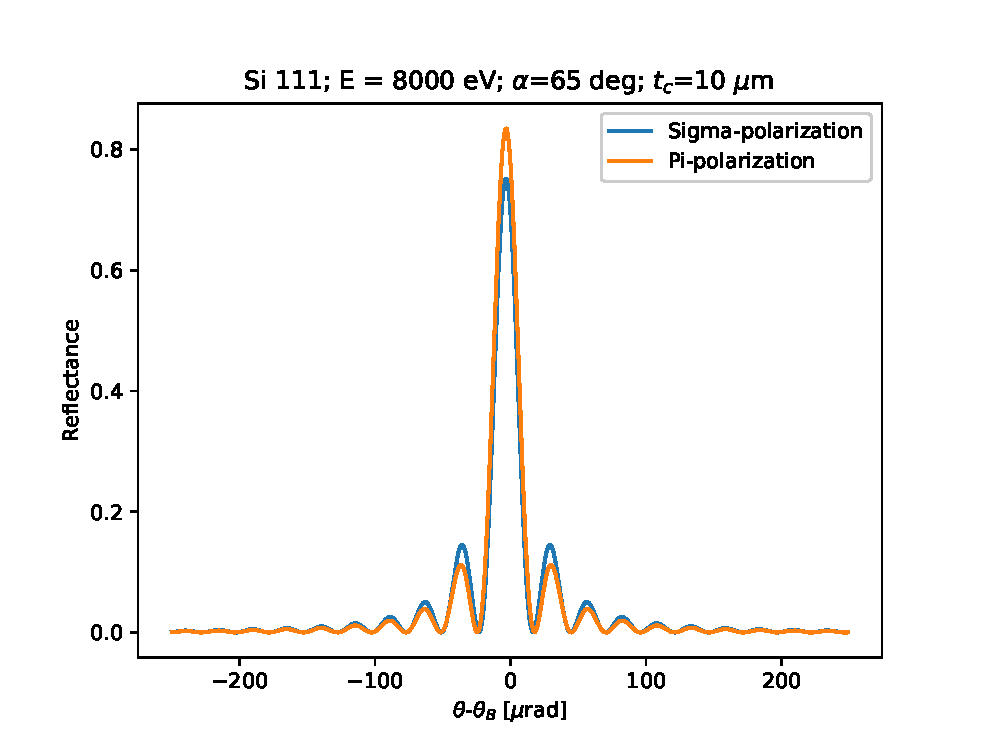
\includegraphics[width=0.49\textwidth]{figures/Laue_1.eps}
    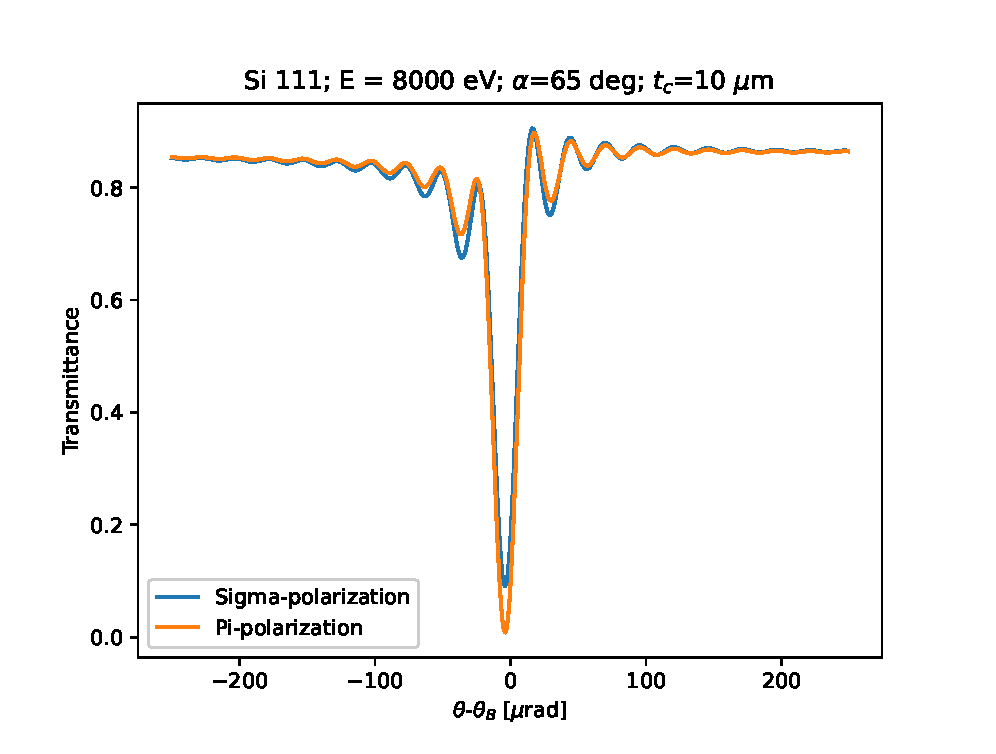
\includegraphics[width=0.49\textwidth]{figures/Laue_2.eps}
    \caption{Example of reflectance and transmittance for a Laue Si 111 crystal.}
\end{figure}

\inred{
Note that $a, u_0, \omega$ in equations~(\ref{eq:lauerandt}) are complex. The careful look at the real and imaginary parts conducts to common expressions for absorption and Pendell\"osung. The real part of the exponential argument gives to a pure absorption term:  
$\exp(\operatorname{Re} i s (u_0+\omega))
= \exp(\operatorname{Im} s (u_0 + \omega))$. Using $u_0 + \omega = (1/2)[b(u_0+\alpha')+u_0]$, we find
\begin{equation}
    \exp[\operatorname{Im} s (u_0+\omega)] = \exp[T \gamma_0 \large( \frac{1}{\gamma_0} + \frac{1}{\gamma_h} \large) \operatorname{Im} u_0] = \exp[-\frac{\lambda}{\pi} \frac{t_c}{2} \large( \frac{1}{\gamma_0} + \frac{1}{\gamma_h} \large) \operatorname{Im} \chi_0].
\end{equation}
The Pendell\"osung comes from the pure oscillation of $|\sin(as)|^2$. Knowing the identity $|\sin(x+iy)|^2=\sin^2x + \sinh^2 y$, we get the Pendell\"osung distance along $0s_0$ as 
\begin{equation}
    \Lambda = \frac{\pi}{\operatorname{Re} a}=\frac{\lambda}{\operatorname{Re}\sqrt{b\chi_h\chi_{-h} + w^2}},
\end{equation}
which depends on $\theta$. At $\theta=\theta_c$ we find the usual value $\Lambda=\lambda/(\operatorname{Re}\sqrt{b \chi_h \chi_{-h}})$ 
}


%%%%%%%%%%%%%%%%%%%%%%%%%%%%%%%%%%%%%%%%%%%%%%%%%%%%
%
%%%%%%%%%%%%%%%%%%%%%%%%%%%%%%%%%%%%%%%%%%%%%%%%%%%%
\subsection{Bragg case}
\label{sec:TTsolutionsBragg}

For the Bragg case $b<0$. Considering $T$ the path length of the incident beam in the crystal, a ``normalized" incident beam $D_0(0)=B_0(0)=1$. The boundary conditions are $D_0(0)=B_0(0)=1$ and $D_h(T)=B_h(T)=0$. Introducing the general solutions (\ref{eq:BSolutions}) in equation~(\ref{eq:TTinB}) and applying the boundary conditions we obtain: 
\begin{subequations}
\label{eq:TTbraggCoefficients}
\begin{align}
c_1&=\frac{\xi_2 \exp(-i a T)}{\xi_2\exp(-i a T)-\xi_1 \exp(i a T)}\\
c_2&=\frac{-\xi_1 \exp(i a T)}{\xi_2\exp(-i a T)-\xi_1\exp(i a T)}.
\end{align}
\end{subequations}
We then obtain
\begin{subequations}
\begin{align}
B_h(0)=\xi_1 \xi_2 \frac{\exp(i a T) - \exp(-i a T)}{\xi_1 \exp(i a T) - \xi_2 \exp(-i a T)}=
\frac{-b i u_h \sin(a T)}{a \cos(a T) + i \omega \sin(a T)}\\
B_0(T)= \frac{\xi_1 - \xi_2}{\xi_1 \exp(i a T) - \xi_2 \exp(-i a T)}=
\frac{a}{a \cos(a T) + i \omega \sin(a T)},
\end{align}
\end{subequations}
which in terms of $D$ we get the amplitudes:

\begin{subequations}
\label{eq:braggrandt}
\begin{empheq}[box=\fbox]{align}
r = \frac{D_h(0)}{D_0(0)}=
\frac{-i b u_h \sin(a T)}{a \cos(a T) + i \omega \sin(a T)}\\
t = \frac{D_0(T)}{D_0(0)}= 
\frac{a~\exp(i T (u_0+ \omega))}{a \cos(a T) + i \omega \sin(a T)} ,
\end{empheq}
\end{subequations}

The diffraction profiles are $|r|^2 P$ (diffracted beam or reflectance) and $|t|^2$ (forward diffracted or transmittance).
An example is in Fig.~\ref{fig:braggProfiles}. 

\begin{figure}\label{fig:braggProfiles}
    \centering
    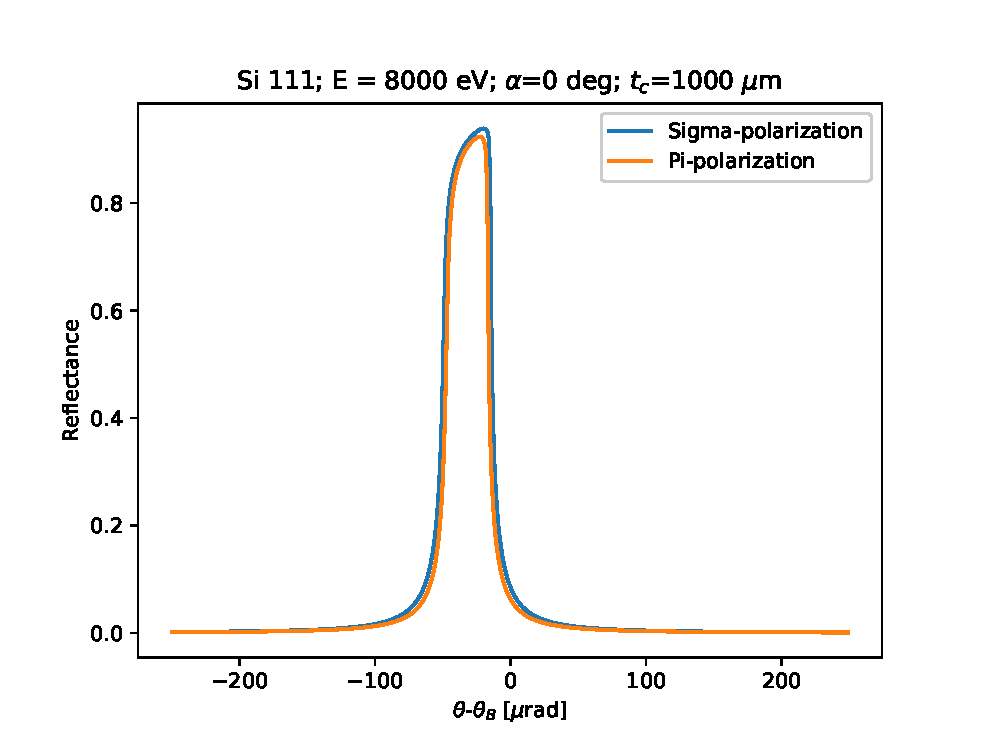
\includegraphics[width=0.49\textwidth]{figures/Bragg_1.eps}
    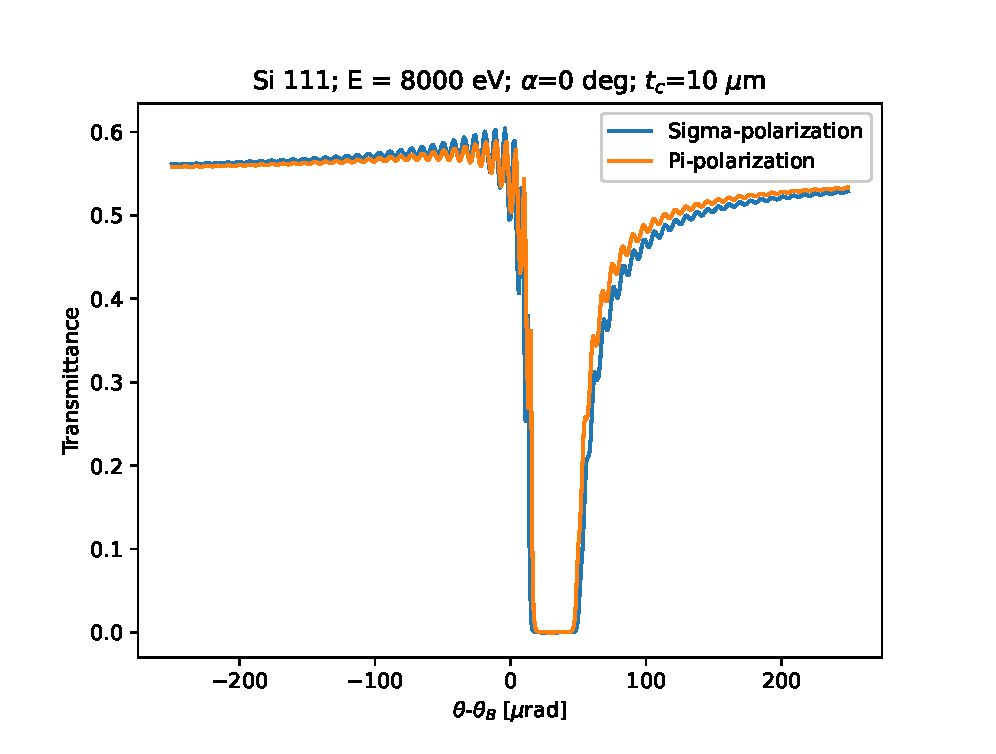
\includegraphics[width=0.49\textwidth]{figures/Bragg_2.eps}
    \caption{Example of reflectance and transmittance for a Bragg Si 111 crystal of $t=$\SI{10}{\micro\meter} at 8 keV. }
\end{figure}


\inblue{A particular case is to consider zero absorption. 
$a^2$ is real negative \todo{Why?} if $|\theta-\theta_c|<|\chi_h|/(|b|^2 \sin(2 \theta_B))$, then $aT=i |a| T$, $\cos(a T)=\cosh(|a|T)$, $\sin(a T)=i \sinh(|a|T)$, 
\begin{equation}
    r = \frac{b u_h \sinh(|a|T)}{i |a|T \cosh(|a|T)- \omega
    \sinh(|a|T)}=
\frac{i |b| u_h \tanh(|a|T)}{|a|+ i \omega \tanh(|a|T)}.
\end{equation}
For $t \rightarrow \infty$, 
\begin{equation}
    r \rightarrow - \frac{i \inred{|b|} u_h}{|a|+ i \omega} .
\end{equation}
}

\inblue{
It is interesting to calculate the field inside the crystal, i.e. $B_0(s)$ and $B_h(s)$. Introducing the coefficients in (\ref{eq:TTbraggCoefficients}) into equations (\ref{eq:BSolutions}) we obtain, after some algebraic manipulation
\begin{subequations}\label{eq:bragginside}
\begin{align}
D_h(s)&=\frac{i b u_h \sin(as - aT)}{a \cos(aT) + i \omega \sin(aT)} e^{is(u_0+\omega)}\\
D_0(s)&= \frac{a \cos(as-aT) - i \omega \sin(as-aT)}{a \cos(aT) + i \omega \sin(aT)} e^{is(u_0+\omega)}.
\end{align}
\end{subequations}
}

\begin{figure}\label{fig:braggMap}
    \centering
    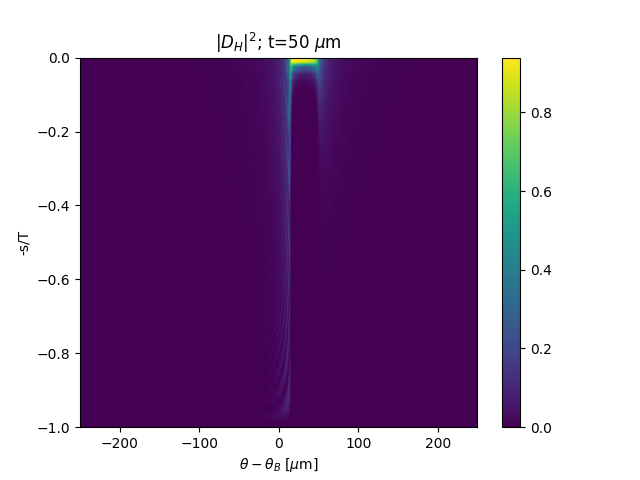
\includegraphics[width=0.49\textwidth]{figures/Bragg_DH.png}
    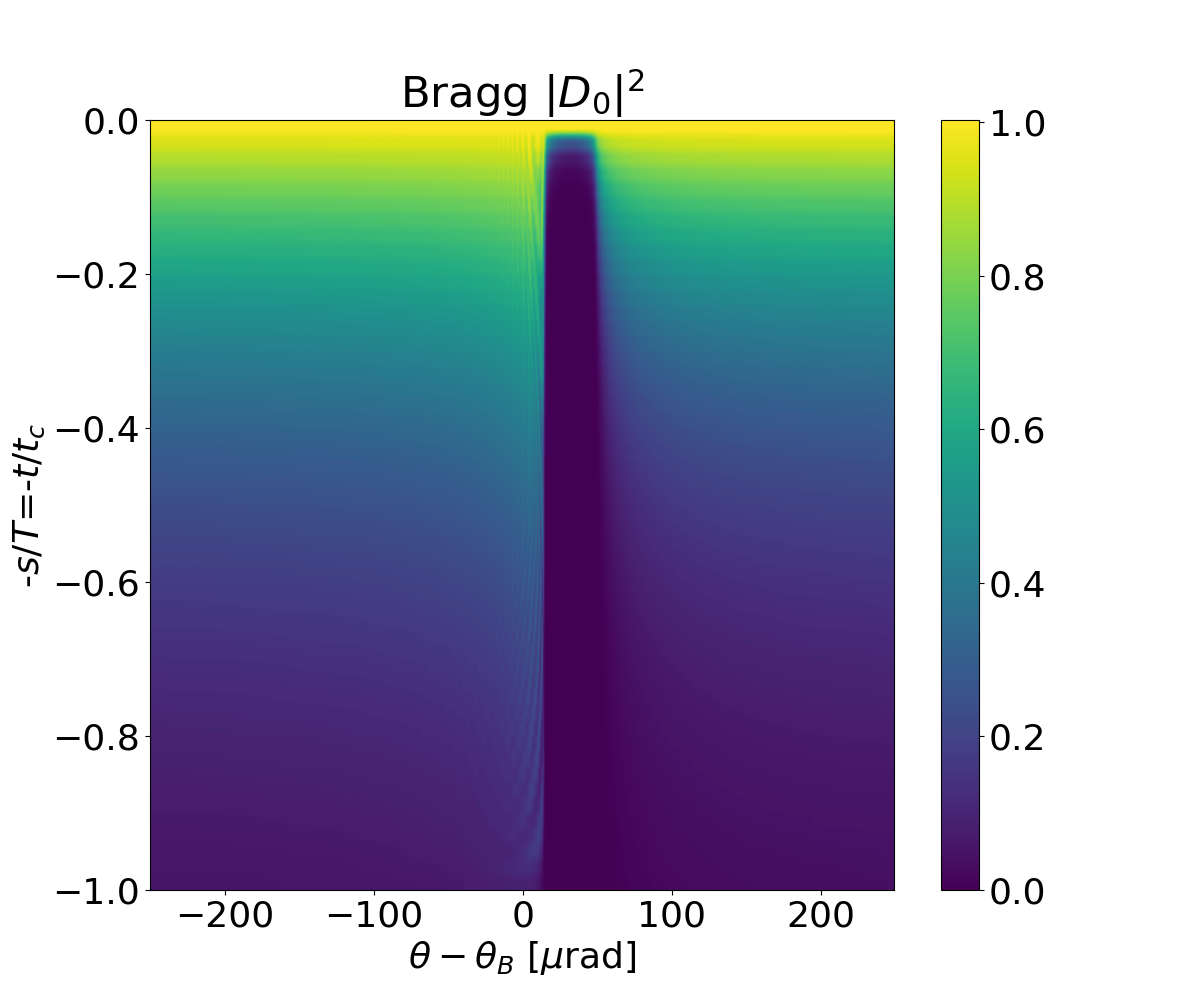
\includegraphics[width=0.49\textwidth]{figures/Bragg_D0.png}
    \caption{Example of intensity of the electric fields inside the crystal as a function of the 
    deviation angle $\theta-\theta_B$ and thickness ratio $-s/T$. 
    Left $|D_h|^2$, right $|D_0|^2$. 
    The crystal is Si 111 at 8 keV with thickness $t=$\SI{10}{\micro\meter}. 
    }
\end{figure}

\todo{Do the same for Laue }

\section{Scattering and transfer matrices}
\label{sec:matrices}

Equations (\ref{eq:BSolutions}) represent a system of two equations containing two coefficients $c_1$ and $c_2$ and two fields ($B_0$ and $B_h$) that are latter expressed at the top ($s=0$) and bottom ($s=T$) surfaces. From these four fields, we can calculate two as a function of the other two. In the usual case, we calculate the diffracted and transmitted fields at the corresponding exit surface (which depends on the geometry, Bragg or Laue) given the other two that are set as boundary conditions. This gives the ``scattering matrix". In other cases, when one considers a complex crystal made by several piled individual crystal layer, we would be interested in calculating the diffracted and transmitted beam at the bottom as a function of the beams from the top.   

\subsection{Scattering matrix in Bragg case}
For the Bragg case, we calculate $D_0(T)$ (transmitted) and $D_h(0)$ (diffracted) as a function of generic $D_0(0)$ and $D_h(T)$, so we can write in matrix form
\begin{equation}
    \begin{pmatrix}
    D_h(0)\\
    D_0(T)
    \end{pmatrix}
    =
    S
        \begin{pmatrix}
    D_0(0) \\
    D_h(T)
    \end{pmatrix}
    =
    \begin{pmatrix}
    s_{11} & s_{12}\\
    s_{21} & s_{22}
    \end{pmatrix}
    \begin{pmatrix}
    D_0(0) \\
    D_h(T)
    \end{pmatrix},
\end{equation}
where the terms of the scattering matrix $S$ are 
\begin{subequations}\label{eq:scatteringMatrixBragg }
\begin{align}
s_{11} &= \frac{-i b u_h \sin(a T)}{a \cos(a T) + i \omega \sin(a T)};\\
s_{12} &= \frac{a~\exp(-i T (u_0+ \omega))}{a \cos(a T) + i \omega \sin(a T)};\\
s_{21} &= \frac{a~\exp(i T (u_0+ \omega))}{a \cos(a T) + i \omega \sin(a T)};\\
s_{22} &= \frac{-i u_{-h} \sin(a T)}{a \cos(a T) + i \omega \sin(a T)}.
\end{align}
\end{subequations}


For the case studied in section~\ref{sec:TTsolutionsBragg} we set $(D_0(0),D_h(T))=(1,0)$ from there we get $s_{11}=r; s_{21}=t$, with $r$ and $t$ from equations (\ref{eq:braggrandt}). Similarly, when the incident beam enters the crystal by the bottom surface, as studied in appendix~\ref{sec:braggfromtheback}, we set $(D_0(0),D_h(T))=(0,1)$ and  we get $s_{12}=\bar{r}; s_{22}=\bar{t}$, with $r$ and $t$ from equations (\ref{eq:braggrbarandtbar}) \todo{suppress the appendix?}.


\subsection{Transfer matrix in Bragg case}
For the Bragg case, we calculate the fields at the bottom surface $(D_0(T),D_h(T))$ as a function of those at the top surface $(D_0(0),D_h(0))$, so we can write in matrix form
\begin{equation}
    \begin{pmatrix}
    D_0(T)\\
    D_h(T)
    \end{pmatrix}
    =
    M
        \begin{pmatrix}
    D_0(0) \\
    D_h(0)
    \end{pmatrix}
    =
    \begin{pmatrix}
    m_{11} & m_{12}\\
    m_{21} & m_{22}
    \end{pmatrix}
    \begin{pmatrix}
    D_0(0) \\
    D_h(0)
    \end{pmatrix},
\end{equation}
where the terms of the transfer matrix $M$ are 
\begin{subequations}\label{eq:scatteringMatrixBragg }
\begin{align}
m_{11} &= \left[ \cos(aT)-i\frac{\omega}{a}\sin(aT) \right] \inred{\exp(i T (u_0+\omega))};\\
m_{12} &= i u_{-h}\frac{\sin(aT)}{a} \inred{\exp(i T (u_0+\omega))};\\
m_{21} &= i b u_h \frac{\sin(aT)}{a} \inred{\exp(i T (u_0+\omega))};\\
m_{22} &= \left[ \cos(aT)+i \frac{\omega}{a}\sin(aT) \right] \inred{\exp(i T (u_0+\omega))}.
\end{align}
\end{subequations}

It can be verified that $M^2$ is of the same form as $M$ where $T$ is replaced by $2T$. 

\todo{ Some possible ideas for the continuation of the matrix methods
\begin{itemize}
    \item the multilayer case:
    \begin{itemize}
        \item the Parratt recursion formula
        \item transition layer (non-abrupt change, see \cite{Lobach})
        \item Roughness layer
    \end{itemize}and 
    \item relation between scattering and transfer matrices. Can be built a multilayered $M=\Pi M_i$ and then calculate its corresponding scattering matrix?
    \item may be: discuss the roughness layer
    \item may be: discuss the grazing incidence case (\cite{Yashiro2001, Stepanov1998})
\end{itemize}
}


% \begin{figure}\label{fig:2T}
%     \centering
%     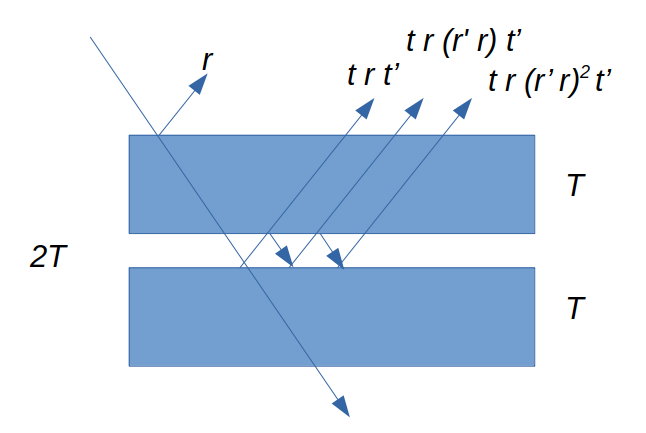
\includegraphics[width=0.49\textwidth]{figures/fig2T.png}
%     \caption{A $2T$ crystal made with two $1T$ crystals. \todo{replace $r'$ by $\bar r$ and $t'$ by $\bar t$}}
% \end{figure}

% As a consistency test, we consider a single Bragg crystal of $s=2T$ made by two piled crystals of $T$. The reflectance $r_{2T}$ of the 2$T$ crystal is (see Fig.~\ref{fig:2T})
% \begin{equation}
%     r_{2T} = r+t r \bar t  \sum_{n=0}^\infty (r \bar r)^n =r + \frac{t r \bar t}{1-r \bar r} = r \frac{1-r \bar r + t \bar t}{1-r \bar r}
% \end{equation}


% We define $b=\sin\theta_0/\sin\theta_h$ ($\theta_{0,h}$ the grancing angles of the incident and reflected directions with respect to the crystal surface, and $s=s_0+s_h/b$. Unlike the usual convention, we have $b>0$. The crystal surface has equation $s=0$. 

% The refractive wave is such that $D_0^{\text{ref}}=\exp(u_0 s_0) f(s_h)$, with $D_0^{\text{ref}}(s_h/b,s_h)=1$; therefore $\exp(i u_0 s_h/b)=1$ and $D_0^{\text{ref}}=\exp(i u_0 (s_0 - s_h/b) )=\exp(i u_o s)$; this implies $Im(u_0)>0$.


% The TT equations are then
% \begin{subequations}
% \label{eq:TTlaue}
% \begin{align}
% D'_0(s) =& i u_0 D_0(s) + i u_{-h} D_h(s); \\
% D'_h(s) =& -i b (u_0 + \alpha') D_h(s) - i b u_{h} D_0(s).
% \end{align}
% \end{subequations}

% We introduce the functions $B_{0,h}(s)$ by setting
% \begin{equation}
% \label{eq:TTbraggB}
% D_{0,h} = \exp \left( i s \frac{u_0 - b (u_0+\alpha')}{2} \right) B_{0,h} = \exp(i s (u_0-\omega)) B_{0,h},  
% \end{equation}
% with $\omega=(b(u_0+\alpha')+u_0))/2$. 

% \inblue{Note that $\exp(i s (u_0 - \omega))=\exp(-s(1+b)/2+ b \alpha/2))=\exp(-s(1+b)/2+ b \sin(2 \theta_B) (\theta - \theta_c)))$, with the corrected value of the Bragg angle $\theta_c=\theta_s - \frac{(1+b) Re(\chi_0)}{2 b \sin(2 \theta_B)}$
% }



% They are solutions of 
% \begin{subequations}
% \begin{align}
% B'_0(s) =& -i \omega B_0(s) + i u_{-h} B_h(s); \\
% B'_h(s) =& i \omega B_h(s) + i b u_{h} B_0(s).
% \end{align}
% \end{subequations}

\newpage
\todo{
\begin{itemize}
    \item direction of the output planewave
    \item matrices for Laue case
    \item discuss the fact that $b$ is not constant.
\end{itemize}
}

%%%%%%%%%%%%%%%%%%%%%%%%%%%%%%%%%%%%%%%%%%%%%%%%%%%%
%
%%%%%%%%%%%%%%%%%%%%%%%%%%%%%%%%%%%%%%%%%%%%%%%%%%%%
\inred{
\section{New possible sections}
\subsection{The crystalpy library}
\subsection{Crystal examples}
\begin{itemize}
    \item rocking curves (see Figs.~\ref{fig:braggProfiles}, \ref{fig:laueProfiles})
    \item differences with Darwin (see \cite{Yashiro2000, Yashiro2001}), Ewald, Zachariasen, etc. 
    \item field maps inside the crystal using equation~(\ref{eq:bragginside})
    \item skew scans (2D scans) [Needs to calculate the output direction]
    \item crystal curvature/deformation treated with matrices??
    \item extend the matrices to include s and p polarization to calculate polarization changes
\end{itemize}

\subsection{Multilayer examples }
(\cite{Osterhoff2012, Osterhoff2013})
\section{Conclusions and future perspectives}
\label{sec:summary}

}

% \ack{Acknowledgements}
% A large part of this work comes from ...


\bibliography{iucr} % reads iucr.bib with items
\bibliographystyle{iucr}
%\referencelist{library}

\appendix

\section{Derivation of the TT equations for a rotating perfect crystal}
\label{appendix:rotating}

In the ``rotating crystal mode", the crystal is rotated around an axis perpendicular to the ``diffraction plane" which contains the diffraction vector $\textbf{h}$ and the wave-vector $\textbf{k}_0$ of the fixed incident plane-wave in vacuum. The crystal rotation from the exact geometrical Bragg position may be viewed as a special kind of crystal deformation. We propose to use the Takagi-Taupin approach to derive some basic results of the usual dynamic theory for the perfect crystal diffraction. 

The x-ray wavefield inside the crystal is set as
\begin{subequations}
\label{eq:wavefieldappendix}
\begin{align}
        \Psi(\textbf r) = 
        e^{i \textbf k_0 . \textbf r} \left[
        A_0(\textbf r) + e^{i \textbf k_{B} . \textbf r} A_h(\textbf r)
        \right] = 
        \nonumber\\
        A_0(\textbf r) e^{i \textbf k_0 . \textbf r} + A_{h}(\textbf r) e^{i \textbf k_{hB} . \textbf r},
\end{align}
\end{subequations}
$\textbf{h}_B$ representing the diffraction vector in exact Bragg position. The vector $\textbf k_{hB}$  is therefore such that $|\textbf k_{0}|=|\textbf k_{hB}|=k=2 \pi / \lambda$. The Fourier coefficients $\chi_h$ of the perfect crystal susceptibility are \cyan{to be} replaced by the function $\chi_h \exp[i\textbf{k}_b.\textbf{u}(\textbf{r})]$, in which $\textbf{u}(\textbf{r})$ is the displacement field of the rotated crystal. The phase term $\exp[i\textbf{h}_B.\textbf{u}(\textbf{r})]$ will be written as $\exp(i\phi(\textbf{r})$. In such conditions, the following form of the TT equations
\begin{subequations}
\label{eq:TTvectorappendix}
\begin{align}
2 i \textbf{k}_0 . \nabla A_0 + \chi_0 k^2 A_0 + \chi_{-h} k^2 \exp(i\phi) A_h =& 0; \\
2 i \textbf{k}_{hB} . \nabla A_h + \chi_0 k^2 A_h + \chi_{h} k^2 \exp(-i\phi) A_0 =& 0,
\end{align}
\end{subequations}
is obtained by inserting this expression in the \cyan{Helmholz equation~(\ref{eq:helmholz})}, with the following approximations: the 2$^{\text{nd}}$-order derivatives of $A_{0,h}$ supposed to be slowly varying amplitudes are neglected and only the terms containing $\exp(i\textbf{k}_0.\textbf{r})$ in the product $\chi\Psi$ are considered. Introducing oblique coordinates $(s_0,s_h)$ in the diffraction plane, along the directions $\textbf{k}_0$ and $\textbf{k}_{hB}$, so that $\textbf{k}_0.\nabla A_0=k\frac{\partial A_0}{\partial s_0}$ and  $\textbf{k}_{hB}.\nabla A_h=k\frac{\partial A_h}{\partial s_h}$, the TT equations are
\begin{subequations}
\begin{align}
\frac{\partial A_0}{\partial s_0} =& \frac{ik}{2} \left[ \chi_0 A_0+ \chi_{-h} \exp(i\phi) A_h\right]; \\
\frac{\partial A_h}{\partial s_h} =& \frac{ik}{2} \left[ \chi_0 A_h+ \chi_{\cyan{h}} \exp(-\phi) A_0\right].
\end{align}
\end{subequations}

Performing the transformation $A_0=D_0$ and $\exp(i\phi) A_h=D_h$, we obtain
\begin{subequations}
\begin{align}
\frac{\partial D_0}{\partial s_0} =& \frac{ik}{2} \left[ \chi_0 D_0+ \chi_{-h} D_h\right]; \\
\frac{\partial D_h}{\partial s_h} =& \frac{ik}{2} \left[ (\chi_0 + \frac{2}{k}\frac{\partial\phi}{\partial s_h} ) D_h+ \chi_{\cyan{h}} D_0\right].
\end{align}
\end{subequations}
This is identical to equation~(\ref{eq:TT}) considering that $\alpha=\frac{2}{k}\frac{\partial\phi}{\partial s_h}$, \cyan{which demonstration follows.}

\subsection{Demonstration of $\alpha=\frac{2}{k}\frac{\partial\phi}{\partial s_h}$ }

Let $\textbf{i}_{0,h}$ be unit vectors along the directions of $\textbf{k}_0$ an $\textbf{k}_{hB}$; the crystal rotation $\Delta\theta=\theta-\theta_B$ transforms $\textbf{i}_{0,h}$ into $\textbf{j}_{0,h}$. A position vector $s_0\textbf{i}_0+s_h\textbf{i}_h$ is transformed into $s_0\textbf{j}_0+s_h\textbf{j}_h$. The displacement field is $\textbf{u}(s_0,s_h)=s_0(\textbf{j}_0-\textbf{i}_0)+ s_h(\textbf{j}_h-\textbf{i}_h)$; $\textbf{h}_B=k(\textbf{i}_h-\textbf{i}_0)$. Hence
\begin{equation}
    \phi(s_0,s_h)=\textbf{h}_B.\textbf{u}=k s_0(\textbf{i}_h-\textbf{i}_0).(\textbf{j}_0-\textbf{i}_0) + 
    k s_h(\textbf{i}_h-\textbf{i}_0).(\textbf{j}_h-\textbf{i}_h).
\end{equation}
We note that 
\begin{subequations}
\begin{align}
    \textbf{i}_0.\textbf{j}_0=\textbf{i}_h.\textbf{j}_h=&\cos\Delta\theta_B \\
    \textbf{i}_0.\textbf{j}_h=&\cos(2\theta_B +\Delta\theta) \\
    \textbf{i}_h.\textbf{j}_0=&\cos(2\theta_B -\Delta\theta) \\
    \textbf{i}_0.\textbf{i}_h=&\cos2\theta_B
\end{align}
\end{subequations}
therefore, 
\begin{subequations}
\begin{align}
    \frac{2}{k}\frac{\partial\phi}{\partial s_h} =  2(\textbf{i}_h-\textbf{i}_0).(\textbf{j}_h-\textbf{i}_h)= \nonumber\\
    2(\cos\Delta\theta - \cos(2\theta_B+\Delta\theta)-1+\cos2\theta_B)= \nonumber\\
    2[(\cos\Delta\theta-1)(1-\cos2\theta_B)+\sin2\theta_B\sin\Delta\theta]=\nonumber\\
    4 \sin\theta_B[\sin\theta_B(\cos\Delta\theta-1)+\cos\theta_B\sin\Delta\theta]=\nonumber\\
    4 \sin\theta_B[\sin(\theta_B+\Delta\theta)-\sin\theta_B]\approx\nonumber\\
    \alpha
\end{align}
\end{subequations}



%%%%%%%%%%%%%%%%%%%%%%%%%%%%%%%%%%%%%%%%%%%%%%%%%%%%%%%%%%%%%%%%%%%%%%%%%%%%%%%%%%%%%%%%%%%%%%%%%%%%%%%%%%%%%%%%%%%%%%%%%%%%%%%%%%%%%%%%%%%%%%%%%%%%%%%%%%%%%%
\section{Solutions of TT equations (\ref{eq:TTinB}) using the Laplace transform}
\label{appendix:laplace}


\subsubsection{Laue solution based on Laplace transform}
\label{sec:laplaceLaue}
Let denote $\bar{F}(p)$ the Laplace transform of a function $F(s)$
\begin{equation}
\Bar{F}(p) = \int_0^\infty ds \exp(-p s) F(s).
\end{equation}
Applying the Laplace transform to equations~(\ref{eq:TTinB}) we get
\begin{subequations}
\label{eq:TTlaueLaplace}
\begin{align}
(p + i \omega) \bar{B_0}(p) - i u_{-h} \bar{B_h}(p)= & 1 \\
(p - i \omega) \bar{B_h}(p) - i b u_{h} \bar{B_0}(p)= & 0.
\end{align}
\end{subequations}
The solutions are
\begin{subequations}
\begin{align}
\bar{B_0}(p) &= \frac{(p - i \omega) }{p^2 + a^2} \\
\bar{B_h}(p) &= \frac{i b u_h}{p^2 + a^2},
\end{align}
\end{subequations}
with, \inred{as previously defined,} $a^2=\omega^2 + b u_h u_{-h}$, $a=\sqrt{\omega^2+b u_h u_{-h}}$
hence one retrieve the same results of equations (\ref{eq:laueSolutionsB}) using the fact that  $(p^2+a^2)^{-1}$ and $p(p^2+a^2)^{-1}$ are the Laplace transform of \inred{ $\sin(a s)/a$ and $\cos(a s)$}, respectively. 

\todo{ REMOVE (NOT USED)? Using the formula $\sin(p+i q)=\sin p \cos(i q) + \cos p \sin(i q)=\sin p \cosh q + i \cos p \sinh q$. it is shown that $|\sin(a s)|^2=\sin^2(s \operatorname{Re}(a)) + \sinh^2(s \operatorname{Im}(a)$;
}


\subsubsection{Bragg solution based on Laplace transform}By Laplace transform of equation~(\ref{eq:TTinB}), and calling \inred{$r'=B_h(0)$}, we obtain
\begin{subequations}
\label{eq:TTbraggLaplace}
\begin{align}
(p + i \omega) \bar{B_0}(p) - i u_{-h} \bar{B_h}(p)= & 1 \\
(p - i \omega) \bar{B_h}(p) - i u_{h} \bar{B_0}(p)= & r',
\end{align}
\end{subequations}
or 
\begin{subequations}
\begin{align}
\bar{B_0}(p) &= \frac{p - i \omega + i r u_{-h}}{p^2 + a^2} \\
\bar{B_h}(p) &= \frac{r' (p + i \omega) + i b u_h}{p^2 + a^2},
\end{align}
\end{subequations}
with \inred{(the same as before)} $a^2=\omega^2+b u_h u_{-h}$. Hence:
\begin{subequations}
\begin{align}
B_0(s) &= \cos(a s) + i (r u_{-h} - \omega) \frac{\sin(a s)}{a}\\
B_h(s) &= r [\cos(a s) + i \omega \frac{\sin(a s)}{a}] + i b u_h \frac{\sin(a s)}{a}.
\end{align}
\end{subequations}

The $r'$ and then the reflected and transmitted amplitudes are obtained using the condition $D_h(T)=B_h(T)=0$. With some calculation, we obtain: 
\begin{subequations}
\begin{align}
r=\frac{D_h(0)}{D_0(0)} =& B_h(0) = r' = \frac{-i b u_h \sin(a T)}{a \cos(a T) + i\omega \sin(a T)}\\
t =\frac{D_0(T)}{D_0(0)}= & B_0(T) ~ \inred{\exp(i T (u_0+\omega))} = \frac{a~\inred{\exp(i T (u_0+\omega))}}{a \cos(a T) + i\omega \sin(a T)} ,
\end{align}
\end{subequations}
with $a=\sqrt{\omega^2 + b u_h u_{-h}}$, and  
\inred{$T=t_c/\cos(\theta_0)$ with $t_c$ the crystal thickness. }

%%%%%%%%%%%%%%%%%%%%%%%%%%%
%%%%%%%%%%%%%%%%%%%%%%%%%%%
%%%%%%%%%%%%%%%%%%%%%%%%%%%

\section{Bragg amplitudes when beam enters from the back of the crystal}
\label{sec:braggfromtheback}
It is useful to calculate the reflectance and transmitted amplitudes when the beam enters from the back along the $\textbf{k}_h$ direction for then build the amplitudes of a layered crystal (matrix method). 

\subsubsection{Bragg case:} the entrance surface is $s=T$ and the exit is $s=0$. The boundary conditions are $B_h(T)=1$ and $B_0(0)=0$. From equations~(\ref{sec:TTsolutions}) we get
\begin{subequations}
\begin{align}
c_1 = \frac{1}{\xi_1 \exp(i a T) - \xi_2 \exp(-i a T)}\\
c_2 = \frac{-1}{\xi_1 \exp(i a T) - \xi_2 \exp(-i a T)},
\end{align}
\end{subequations}
and 
\begin{subequations}
\begin{align}
B_0(T) = &c_1 \exp{i a T} + c_2 \exp(-i a T)=
\frac{i u_{-h} \sin(a T)}{a \cos(a T)+ i \omega \sin(a T)}\\
B_h(0) = &c_1 \xi_1 + c_2 \xi_2=
\frac{a}{a \cos(a T)+ i \omega \sin(a T)}.
\end{align}
\end{subequations}
In consequence
\begin{subequations}
\label{eq:braggrbarandtbar}
\begin{align}
\bar r = \frac{D_0(T)}{D_h(T)} = &
\frac{i u_{-h} \sin(a T)}{a \cos(a T)+ i \omega \sin(a T)}\\
\bar t = \frac{D_h(0)}{D_h(T)} = &
\frac{a ~ \exp(-i T (u_0+\omega))}{a \cos(a T)+ i \omega \sin(a T)} .
\end{align}
\end{subequations}
As compared with equations~(\ref{eq:braggrandt}) we see now that $-b$ does not appear in $\bar r$, there us $u_{-h}$ instead of $u_h$ and there is a different sign in the exponential of the numerator in $\bar t$. 


% \section{Derivation of the Lens Equation from the phase-factor of the Takagi-Taupin equations}
% \label{appendix:CLE}





     %-------------------------------------------------------------------------
     % The back matter of the paper - acknowledgements and references
     %-------------------------------------------------------------------------

     % Acknowledgements come after the appendices



     % References are at the end of the document, between \begin{references}
     % and \end{references} tags. Each reference is in a \reference entry.

%\begin{references}
%\reference{Author, A. \& Author, B. (1984). \emph{Journal} \textbf{Vol}, first page--last page.}
%\end{references}
%\cite{knuth84}

%\begin{thebibliography}{30}
%\expandafter\ifx\csname natexlab\endcsname\relax\def\natexlab#1{#1}\fi
%\expandafter\ifx\csname bibnamefont\endcsname\relax
%  \def\bibnamefont#1{#1}\fi
%\expandafter\ifx\csname bibfnamefont\endcsname\relax
%  \def\bibfnamefont#1{#1}\fi
%\expandafter\ifx\csname citenamefont\endcsname\relax
%  \def\citenamefont#1{#1}\fi
%\expandafter\ifx\csname url\endcsname\relax
%  \def\url#1{\texttt{#1}}\fi
%\expandafter\ifx\csname urlprefix\endcsname\relax\def\urlprefix{URL }\fi
%\providecommand{\bibinfo}[2]{#2}
%\providecommand{\eprint}[2][]{\url{#2}}
%
%\bibitem[{\citenamefont{Shvyd'ko}(2016)}]{GuigayFerrero2013}
%\bibinfo{author}{\bibfnamefont{Yu.}~\bibnamefont{Shvyd'ko}},
%\bibinfo{journal}{Phys. Rev. Lett.} \textbf{\bibinfo{volume}{116}},
%\bibinfo{pages}{080801} (\bibinfo{year}{2016}).
%
%%\bibitem[{\citenamefont{Guigay and Ferrero}]{ddd}
%%\bibinfo{author}{\bibfnamefont{Jean-Pierre}~\bibnamefont{Guigay}},
%%\bibinfo{author}{\bibfnamefont{Claudio}~\bibnamefont{Ferrero}},
% % \bibinfo{journal}{xxxx} \textbf{\bibinfo{volume}{xx}},
% % \bibinfo{pages}{xx} (\bibinfo{year}{2012}).
%
%\end{thebibliography}

%% Note added by Overleaf: If using bibtex, remove the "references" environment above, and uncomment the following lines.

%\bibliographystyle{iucr}
%\referencelist{iucr}

%      %-------------------------------------------------------------------------
%      % TABLES AND FIGURES SHOULD BE INSERTED AFTER THE MAIN BODY OF THE TEXT
%      %-------------------------------------------------------------------------
% 
%      % Simple tables should use the tabular environment according to this
%      % model
% 
% \begin{table}
% \caption{Caption to table}
% \begin{tabular}{llcr}      % Alignment for each cell: l=left, c=center, r=right
%  HEADING    & FOR        & EACH       & COLUMN     \\
% \hline
%  entry      & entry      & entry      & entry      \\
%  entry      & entry      & entry      & entry      \\
%  entry      & entry      & entry      & entry      \\
% \end{tabular}
% \end{table}
% 
%      % Postscript figures can be included with multiple figure blocks
% 
% \begin{figure}
% \caption{Caption describing figure.}
% 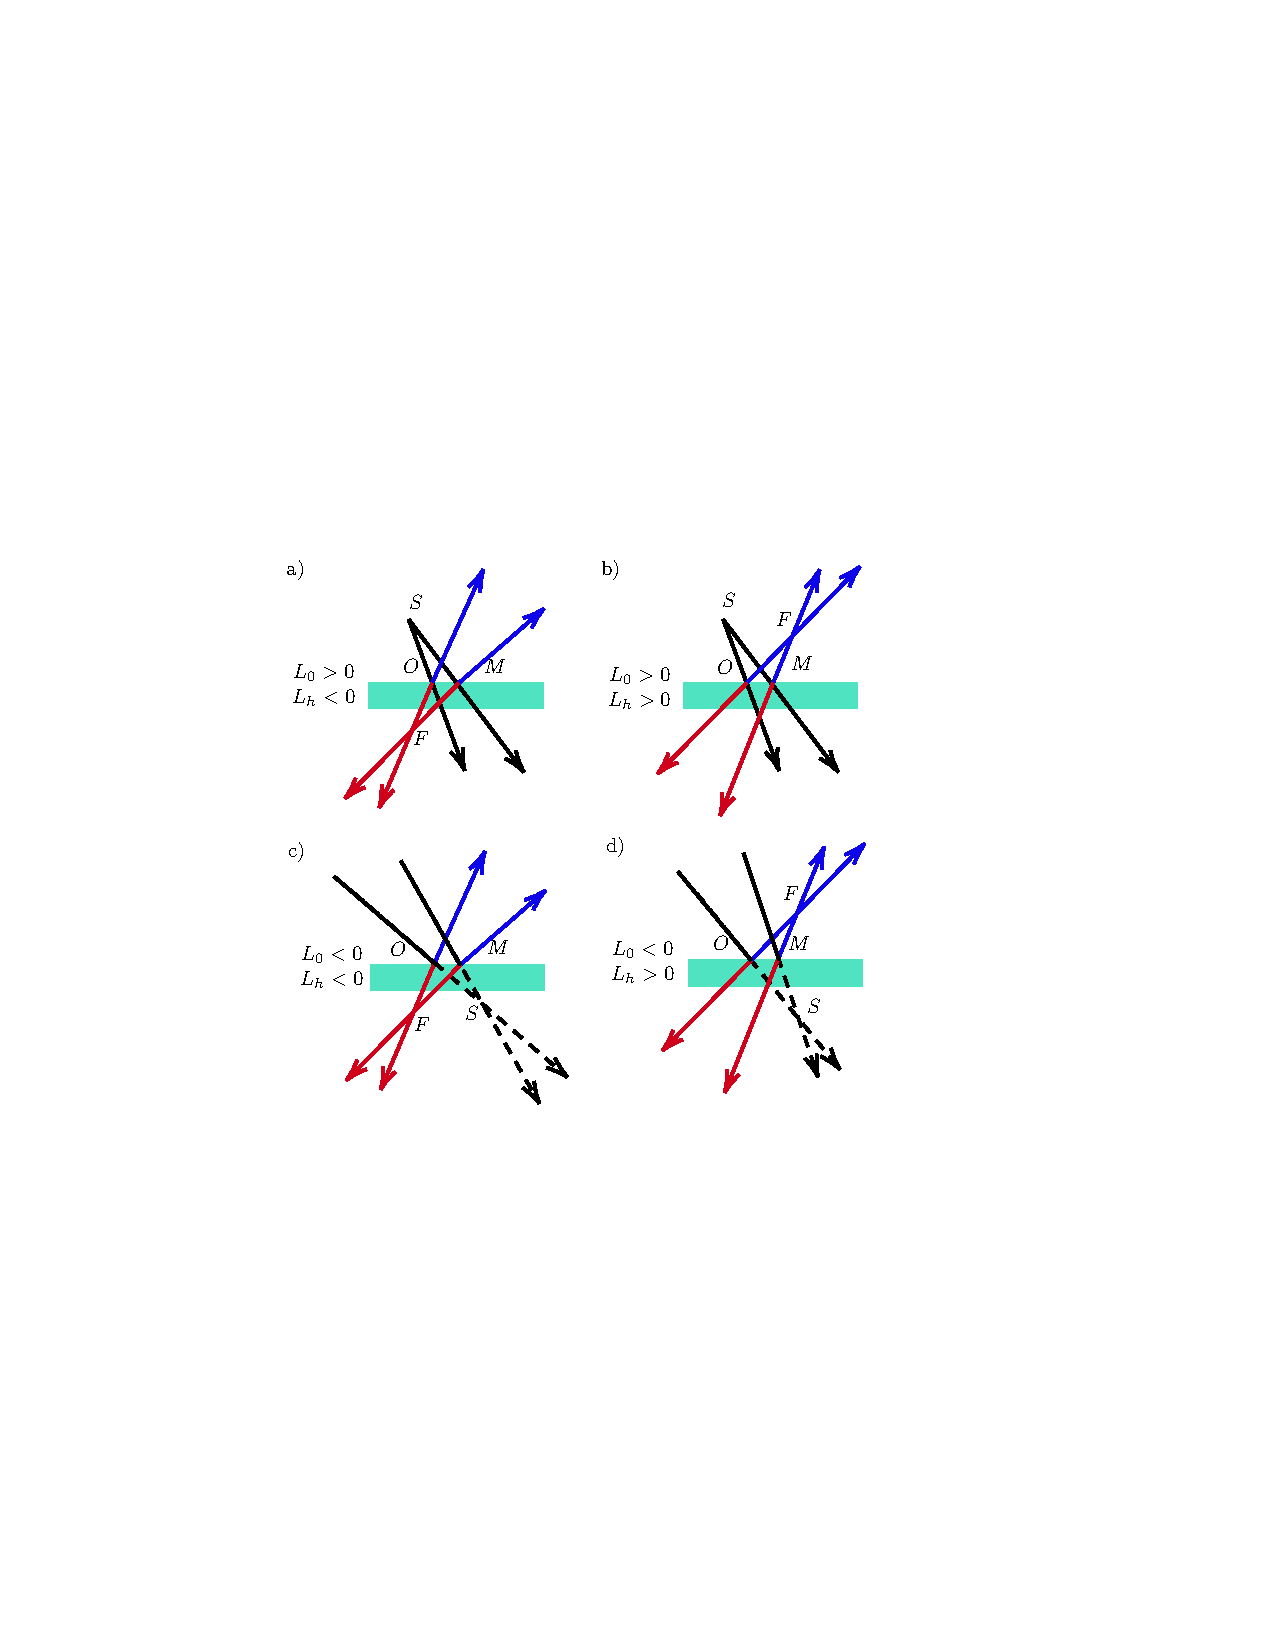
\includegraphics{fig1}
% \end{figure}


\end{document}                    % DO NOT DELETE THIS LINE
%%%%%%%%%%%%%%%%%%%%%%%%%%%%%%%%%%%%%%%%%%%%%%%%%%%%%%%%%%%%%%%%%%%%%%%%%%%%%%
